\documentclass[../main/main.tex]{subfiles}

\toggletrue{student}
\HideSolutionstrue

\raggedbottom

\makeatletter
\renewcommand{\@chapapp}{Induction -- chapitre}
\makeatother

\begin{document}
\setcounter{chapter}{2}
\chapter{Lois de l'induction et induction de \textsc{Neumann}}
\label{ch:loisinduc}

% Dans les chapitres précédents, nous avons vu que le passage d'un courant
% électrique dans un circuit entraînait la création d'un champ magnétique. Ici
% nous étudions la situation opposée~: un champ magnétique peut entraîner la
% création d'un courant électrique.

\section{Le phénomène d'induction}
\label{sec:phinduc}
\subsection{Observations expérimentales}
\label{ssec:inducobsexp}

Soit un solénoïde (bobine longue) non alimenté, relié à un ampèremètre mesurant
le courant qui le traverse. On étudie sa réaction à un champ magnétique dans
deux situations\footnote{Voir l'animation~:
	\url{https://phet.colorado.edu/sims/html/faradays-law/latest/faradays-law_fr.html}}~:

\paragraph*{Bobine dans un champ magnétique constant}~
\smallbreak

\noindent
\begin{minipage}[t]{.4\linewidth}
	~
	\vspace*{-25pt}
	\begin{center}
		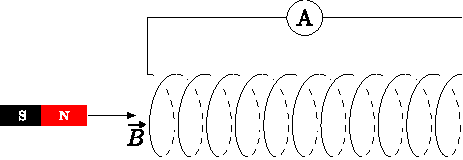
\includegraphics[width=\linewidth]{inducexp1}
		\label{fig:inducexp1}
	\end{center}
\end{minipage}
\hfill
\begin{minipage}[t]{.55\linewidth}
	Les lignes de champ d'un aimant vont de sont Nord vers son Sud. Un champ
	magnétique règne donc dans le solénoïde. On n'observe cependant aucun courant
	dans le solénoïde.
\end{minipage}

\paragraph*{Bobine dans un champ magnétique variable}~
\smallbreak

\noindent
\begin{minipage}[t]{.4\linewidth}
	~
	\vspace*{-25pt}
	\begin{center}
		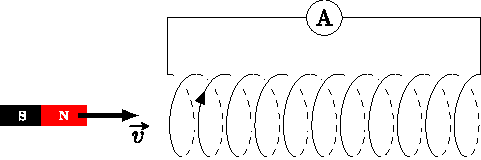
\includegraphics[width=\linewidth]{inducexp2}
		\label{fig:inducexp2}
	\end{center}
\end{minipage}
\hfill
\begin{minipage}[t]{.55\linewidth}
	On déplace l'aimant à proximité de la bobine. On constate qu'\textbf{un
		courant apparaît} dans la bobine, malgré l'absence de générateur.
\end{minipage}

En étudiant le sens du courant induit, on observe que le sens de déplacement de
l'aimant et du courant sont liés~:
\begin{itemize}[label=$\diamond$, leftmargin=10pt]
	\item \cswitch{white}{
		      Sans mouvement relatif, pas de courant.
	      }
	\item \cswitch{white}{
		      Si on approche l'aimant ou le circuit, $i < 0$.
	      }
	\item \cswitch{white}{
		      Si on éloigne l'aimant ou le circuit, $i > 0$.
	      }
\end{itemize}
\smallbreak
De plus,
\begin{itemize}[label=$\diamond$, leftmargin=10pt]
	\item \cswitch{white}{
		      Si on retourne l'aimant, le courant est opposé.
	      }
	\item \cswitch{white}{
		      Plus le mouvement est rapide, plus le courant généré est grand.
	      }
\end{itemize}

\subsection{Bilan}
\label{ssec:inducexpbilan}

\begin{tdefi}{Définition, heart}
	\cswitch{white}{
		Le phénomène d'induction électromagnétique est l'apparition d'une
		\textbf{tension} électrique (et donc à un \textbf{courant} si le circuit est
		fermé) dans un circuit soumis à un champ magnétique dans deux cas de figure~:
	}
	\begin{enumerate}
		\item \cswitch{white}{
			      Lorsque le circuit est plongé dans un champ magnétique \textbf{variable}~:
			      induction de \textsc{Neumann}~;
		      }
		\item \cswitch{white}{
			      Lorsque le circuit est \textbf{déformé} dans un champ magnétique
			      constant~: induction de \textsc{Lorentz} (voir chapitre suivant).
		      }
	\end{enumerate}
\end{tdefi}

Le sens du courant obtenu est donné par la \textbf{loi de \textsc{Lenz}}~:
\begin{tprop}{Loi de modération de \textsc{Lenz}, heart}
	\begin{center}
		\cswitch{white}{
			L'induction modère, par ses conséquences, les causes qui lui a donné
			naissance.
		}
	\end{center}
\end{tprop}

\begin{itemize}[label=$\diamond$, leftmargin=10pt]
	\litem{\textsc{Neumann}}~: courant induit créé un nouveau champ $\vv{B_i}$ qui
	contrecarre les \textbf{variations} de $\vv{B}$ initial~;
	\litem{\textsc{Lorentz}}~: courant induit créé un nouveau champ $\vv{B_i}$ qui
	impose une force s'opposant à la \textbf{déformation}.
\end{itemize}

\begin{rexem}{Application}
	Dans chacun des circuits ci-dessous, la spire circulaire et/ou l'aimant droit
	sont déplacés dans le sens indiqué par la double flèche. Indiquer le signe du
	courant $i$ apparaissant dans la spire pendant le déplacement.
	\begin{center}
		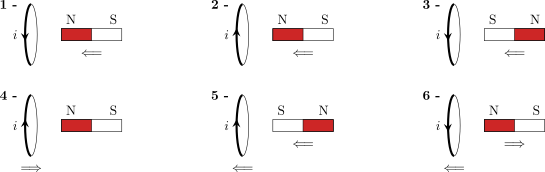
\includegraphics[scale=1]{inducsigne}
		\label{fig:inducsigne}
	\end{center}
	\tcblower
	\cswitch{white}{
		Les lignes de champ vont du Nord vers le Sud. On doit déterminer le sens de
		variation du champ vu par la spire~: le champ induit atténue cette variation.
		On en déduit le signe réel de $i$ par la règle de la main droite.
		\smallbreak
	}
	\begin{side}{}
		\cswitch{white}{
			\begin{enumerate}
				\item
				      $\vv{B}_{\rm aimant}$ augmente vers la gauche~: $\vv{B}_{\rm
						      induit}$ est vers la droite, donc issu de $i_{\rm ind} > 0$.
				      \begin{center}
					      \switch{
						      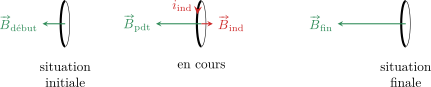
\includegraphics[width=\linewidth]{inducsigne_a}
						      \label{fig:indsa}
					      }{
						      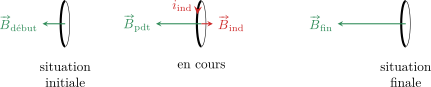
\includegraphics[width=\linewidth, draft=true]{inducsigne_a}
						      \label{fig:indsa}
					      }
				      \end{center}
				\item
				      Même situation physique, convention opposée~: $i_{\rm ind} < 0$.
				\item
				      Cette fois $\vv{B}_{\rm aimant}$ augmente vers la droite~:
				      $\vv{B}_{\rm ind}$ est vers la gauche. Sens réel du courant opposé~:
				      $i_{\rm ind} < 0$.
				      \begin{center}
					      \switch{
						      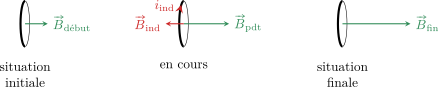
\includegraphics[width=\linewidth]{inducsigne_b}
						      \label{fig:indsb}
					      }{
						      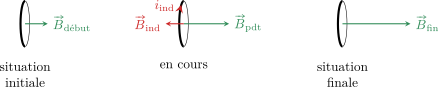
\includegraphics[width=\linewidth, draft=true]{inducsigne_b}
						      \label{fig:indsb}
					      }
				      \end{center}
			\end{enumerate}
		}
		\tcblower
		\cswitch{white}{
			\begin{enumerate}[start=4]
				\item \cswitch{white}{
					      Pareil qu'à la question 2~: $i_{\rm ind} < 0$.
				      }
				\item \cswitch{white}{
					      Pas de mouvement relatif donc pas de variation de champ donc pas
					      d'induction~: $i_{\rm ind} = 0$.
				      }
				\item \cswitch{white}{
					      Mouvement relatif amplifié. Ici, le champ \textbf{diminue} vers la
					      gauche, donc le champ induit le \textbf{renforce}~; ainsi $i_{\rm ind} <
						      0$.
				      }
				      \begin{center}
					      \switch{
						      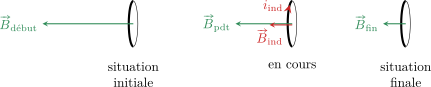
\includegraphics[width=\linewidth]{inducsigne_c}
						      \label{fig:indsc}
					      }{
						      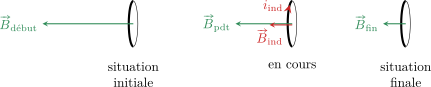
\includegraphics[width=\linewidth, draft=true]{inducsigne_c}
						      \label{fig:indsc}
					      }
				      \end{center}
			\end{enumerate}
		}
	\end{side}
\end{rexem}

\section{Flux magnétique, loi de \textsc{Faraday}}
\label{sec:fluxfara}

\subsection{Flux magnétique}
\label{ssec:flux}
\begin{tdefi}{Définition, heart}
	\cswitch{white}{
		Soit $S$ une surface \textbf{plane}, délimitée par un contour \textbf{orienté}
		par le sens réel du courant, telle que $\vv{S} = S\,\vv{n}$ avec $\vv{n}$
		unitaire normal au plan de sens lié au courant par la main droite. Soit
		$\vv{B}(t)$ le champ magnétique \textbf{uniforme} qui la traverse.
	}
	\smallbreak
	\noindent
	\hfill
	\begin{minipage}[t]{.2\linewidth}
		\begin{center}
			\switch{
				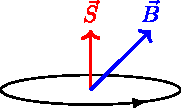
\includegraphics[scale=1]{fluxdef}
				\label{fig:fluxdef}
			}{
				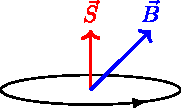
\includegraphics[scale=1, draft=true]{fluxdef}
				\label{fig:fluxdef}
			}
		\end{center}
		\hfill
	\end{minipage}
	\noindent
	\begin{minipage}[t]{.2\linewidth}
		\begin{center}
			\switch{
				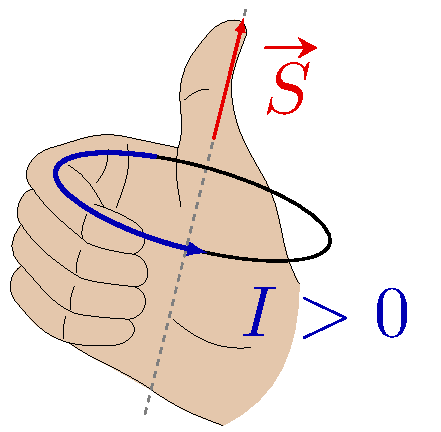
\includegraphics[height=2cm]{ra_surface}
				\label{fig:rasurf}
			}{
				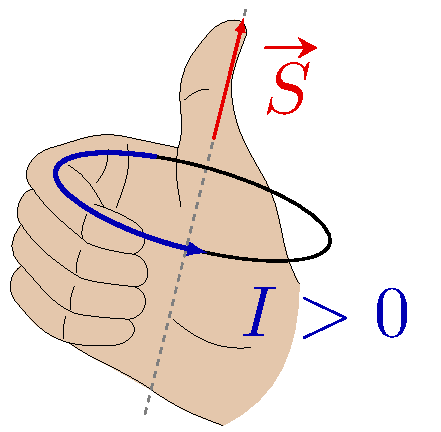
\includegraphics[height=2cm, draft=true]{ra_surface}
				\label{fig:rasurf}
			}
		\end{center}
	\end{minipage}
	\hfill~
	\smallbreak
	\cswitch{white}{
		On appelle \textbf{flux} de $\vv{B}$ à travers $S$ la grandeur
		\textbf{scalaire} $\F_S(\vv{B})$ telle que
		\[
			\boxed{\F_S(\vv{B}) = \vv{B}\cdot \vv{S}}
		\]
		\vspace*{-10pt}
	}
\end{tdefi}

\begin{rrema}{\includehand{-90}{.8cm}}
	Au travers de $N$ spires parcourues par le même champ $\vv{B}$, on a
	\cswitch{white}{
		\[
			\F(t) = N\times \vv{B}\cdot \vv{S}
		\]
		\vspace*{-20pt}
	}
\end{rrema}

On se limite à la description des cas où le champ magnétique est
\textbf{uniforme} à l'échelle de de la situation pour une surface
\textbf{plane}. Dans un cas plus général, il faudrait effectuer une double
intégration sur la surface, en la découpant en éléments infinitésimaux
$\dd{S}(\Mr)$ avec $\Mr \in S$~:
\[
	\F_S(\vv{B}) = \iint _{\Mr \in S}^{} \dd{\F(\Mr)} = \iint _{\Mr \in S}^{}
	\vv{B}(\Mr)\cdot \dd{\vv{S}(\Mr)}
\]

\begin{rexem}{Application}
	Déterminer le flux au travers de la spire circulaire de rayon $R$ plongée dans
	$\vv{B}$ uniforme dans les 4 situations suivantes~:
	\begin{center}
		\begin{tabularx}{\linewidth}{Y|Y|Y|Y}
			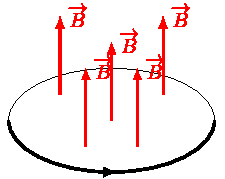
\includegraphics[width=\linewidth]{fluxexo_a} &
			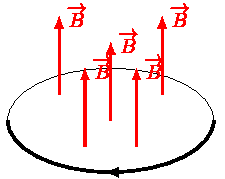
\includegraphics[width=\linewidth]{fluxexo_b} &
			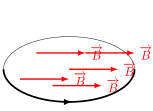
\includegraphics[width=\linewidth]{fluxexo_c} &
			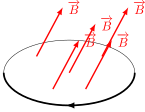
\includegraphics[width=\linewidth]{fluxexo_d}          \\
			\cswitch{white}{
				$\vv{S}\cdot \vv{B} > 0 \Ra \F_S(\vv{B}) = BS$
			}
			                                              &
			\cswitch{white}{
				$\vv{S}\cdot \vv{B} < 0 \Ra \F_S(\vv{B}) = -BS$
			}
			                                              &
			\cswitch{white}{
				$\vv{S}\cdot \vv{B} = 0 \Ra \F_S(\vv{B}) = 0$
			}
			                                              &
			\cswitch{white}{
				$\vv{S}\cdot \vv{B} = -BS\cos{\theta} = \F_S(\vv{B})$
			}
			\\
			                                              &   &  & \\
		\end{tabularx}
	\end{center}
\end{rexem}

\subsection{Loi de \textsc{Faraday}}
\label{ssec:fara}
\begin{tprop}{Loi de \textsc{Faraday}, heart}
	\cswitch{white}{
		Soit un circuit électrique \textbf{fermé} et \textbf{orienté par une
			intensité} soumis à l'action d'un champ magnétique $\vv{B}$. Toute variation
		du flux $\F_S(\vv{B})$ dans ce circuit y fait apparaître une force
		électromotrice (tension à vide) induite $e$, \textbf{orientée dans le même
			sens que $i$}, telle que
		\[
			\boxed{e_{\rm ind}(t) = -\dv{\F}{t}}
		\]
		Électriquement, le système se comporte comme si on y avait mis un générateur
		électrique idéal de f.é.m.\ $e$.
		\smallbreak
		% \vspace*{-0pt}
		\hfill
		\noindent
		\begin{minipage}[c]{.4\linewidth}
			~
			\begin{center}
				\switch{
					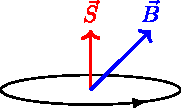
\includegraphics[scale=1]{fluxdef}}{
					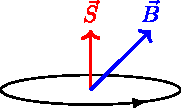
\includegraphics[scale=1, draft=true]{fluxdef}
				}
				\label{fig:fluxdef2}
				\smallbreak
				Circuit physique.
				\smallbreak
				$\vv{S}$ \textbf{orientée avec $i$}.
			\end{center}
		\end{minipage}
		\hfill
		\begin{minipage}[c]{.4\linewidth}
			~
			\begin{center}
				\switch{
					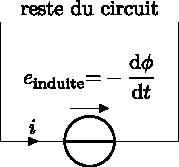
\includegraphics[scale=1]{faraelec}}{
					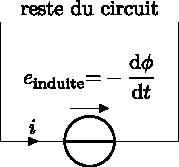
\includegraphics[scale=1, draft=true]{faraelec}
				}
				\label{fig:faraelec}
				\smallbreak
				Modèle électrique.
				\smallbreak
				$i_{\rm ind}$ et $e_{\rm ind}$ \textbf{dans le même sens}.
			\end{center}
		\end{minipage}
		\hfill~
	}
\end{tprop}

\begin{rrema}{Remarques}
	\begin{enumerate}
		\item \cswitch{white}{
			      La f.é.m. $e$ est orientée dans le même sens que le courant $i$, donc
			      en convention \textbf{générateur}~;
		      }
		\item \cswitch{white}{
			      Le signe «~-~» donne la loi de \textsc{Lenz}, et découle en fait de la
			      conservation de l'énergie.
		      }
		\item \cswitch{white}{
			      Si le flux ne varie pas, alors il n'y a pas de force électromotrice.
		      }
	\end{enumerate}
\end{rrema}

\begin{rexem}{Application}
	\noindent
	\begin{minipage}[t]{.7\linewidth}
		On considère un circuit carré de côté $a$ et de résistance totale $R$, situé
		dans un plan orthogonal à un champ magnétique uniforme mais \textbf{variable}
		$\vv{B}(t) = B_0\exr^{-t/\tau}\uz$ avec $B_0$ et $\tau$ strictement positifs.
		Un phénomène d'induction se produit-il dans le circuit~? Si oui, exprimer
		l'intensité $i$ du courant induit représenté sur le schéma, et vérifier que
		son signe soit en accord avec la loi de \textsc{Lenz}.
	\end{minipage}
	\hfill
	\begin{minipage}[t]{.29\linewidth}
		~
		\vspace*{-20pt}
		\begin{center}
			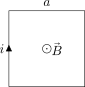
\includegraphics[scale=1]{faraexo}
			\label{fig:faraexo}
		\end{center}
	\end{minipage}
	\tcblower
	\cswitch{white}{
		Le flux à travers le circuit de surface $S = a^2$ est variable puisque le
		champ magnétique l'est. Il y a donc un phénomène d'induction. On a alors~:
		\begin{gather*}
			\begin{aligned}{}
				\F_S(\vv{B}) & = -Ba^2
				\\
				             & = -B_0a^2\exr^{-t/\tau}
			\end{aligned}
			\qqso
			\begin{aligned}{}
				e_{\rm ind}         & = -\dv{\F}{t}
				\\\Lra
				\Aboxed{e_{\rm ind} & = -\frac{B_0a^2}{\tau}\exr^{-t/\tau} < 0}
			\end{aligned}
		\end{gather*}
		Or, comme le circuit est fermé,
		\begin{align*}
			e_{\rm ind}         & = Ri_{\rm ind}
			\\\Lra
			\Aboxed{i_{\rm ind} & = -\frac{B_0a^2}{T\tau}\exr^{-t/\tau} < 0}
		\end{align*}
		donc l'intensité est \textbf{négative}. En effet, le champ magnétique induit
		réel doit s'opposer à la diminution du champ extérieur $\vv{B}$, en créant un
		champ magnétique positif selon $\uz$~: le sens réel du courant donné par la
		main droite est l'opposé de celui représenté.
		\vspace*{-10pt}
	}
\end{rexem}

\section{Phénomène d'autoinduction}
\label{sec:autoind}

\subsection{Flux propre}
\label{ssec:fpropre}
Lorsqu'un courant circule dans une bobine, il créé un champ magnétique. Or, ce
champ créé contribue au flux magnétique total à travers le circuit, et génère
une force électromotrice d'induction~:
\begin{tdefi}{Définition}
	\cswitch{white}{
		Lors de l'étude de l'induction dans un circuit, on différencie le champ créé
		par le circuit, dit \textbf{champ propre}, des autres champs issus d'autres
		sources~:
		\[
			\boxed{\vv{B_{\rm tot}} = \vv{B_{\rm propre}} + \vv{B_{\rm ext}}}
		\]
		\vspace*{-10pt}
	}
\end{tdefi}
Pour une bobine, le champ magnétique propre est celui créé par le courant que
nous avons déjà vu~:
\[
	\vv{B_{\rm propre}}(t) = \mu_0 \frac{N}{\ell }i(t)\,\uz
\]
Le champ magnétique extérieur est lié à la présence d'autres sources au
voisinage (champs de fils électriques par exemple.)

\begin{tdefi}{Définition, heart}
	\noindent
	\begin{minipage}[t]{.7\linewidth}
		\begin{center}
			\cswitch{white}{
				On appelle \textbf{flux propre} noté $\F_p$ d'un circuit le flux de son
				champ magnétique propre $\vv{B_p}$ à travers lui-même.
				\bigbreak
				\danger\ $\F_p \neq \vv{B_p}\cdot \vv{S}$ car \textbf{le champ propre
					n'est pas uniforme} \danger\
			}
		\end{center}
	\end{minipage}
	\hfill
	\begin{minipage}[t]{.29\linewidth}
		~
		\vspace*{-20pt}
		\begin{center}
			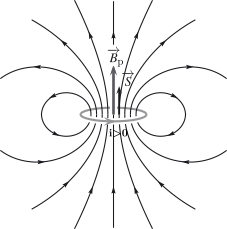
\includegraphics[height=2cm]{fpropre}
			\label{fig:fpropre}
		\end{center}
	\end{minipage}
\end{tdefi}

\subsection{Auto-inductance}
\label{ssec:autoind}
\begin{tprop}{Propriété, heart}
	\cswitch{white}{
		On admet que le flux propre dans un circuit est \textbf{proportionnel à
			l'intensité} du courant dans le circuit, tel que
		\[
			\F_p(t) = Li(t)
		\]
		avec $L$ l'\textbf{inductance propre} (ou auto-inductance) du circuit.
	}
	\begin{itemize}[label=$\diamond$, leftmargin=10pt]
		\item \cswitch{white}{
			      $L > 0$ car $i$ et $\vv{B_p}$ sont orientés par la main droite.
		      }
		\item \cswitch{white}{
			      $L$ ne dépend que de la \textbf{taille} et \textbf{forme} du circuit.
		      }
		\item \cswitch{white}{
			      $L$ s'exprime en henry (\si{H}).
		      }
	\end{itemize}
\end{tprop}

\begin{rexem}{Application}
	Calcul de l'inductance propre d'une bobine. On donne le champ propre
	$\vv{B_p}$ créé dans un solénoïde~:
	\[
		\vv{B_p}(t) = \mu_0 \frac{N}{\ell }i(t)\,\uz
	\]
	% TODO: figure solénoïde avec i dans le bon sens pour student
	\begin{enumerate}
		\item Le sens du courant étant donné, indiquer le sens du champ magnétique.
		      \smallbreak
		      \cswitch{white}{
			      \noindent
			      \begin{minipage}[t]{.4\linewidth}
				      ~
				      \begin{center}
					      \switch{
						      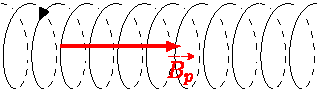
\includegraphics[scale=1]{bobib}
						      \label{fig:bobib}
					      }{
						      
\includegraphics[scale=1]{bobi}
						      \label{fig:bobi}
					      }
				      \end{center}
			      \end{minipage}
			      \hfill
			      \begin{minipage}[t]{.69\linewidth}
				      \vspace*{15pt}
				      $i$ et $\vv{B_p}$ respectent la règle de la main droite.
			      \end{minipage}
		      }
		\item Exprimer le flux du champ magnétique.
		      \smallbreak
		      \cswitch{white}{
			      Pour $N$ spires~:
			      \[
				      \F_p = N\times \vv{B_p}\cdot \vv{S}
			      \]
			      Or, $\vv{B_p}$ et $\vv{S}$ sont tous deux orientés à partir de $i$ selon
			      la règle de la main droite, donc
			      \begin{gather*}
				      \vv{S} = S\uz
				      \qqet
				      \vv{B_p} = \mu_0 \frac{N}{\ell }i(t)\,\uz
				      \\\Lra
				      \boxed{\F_p = \mu_0 \frac{N^2}{\ell }Si(t)}
			      \end{gather*}
		      }
		\item En déduire l'expression de l'inductance propre.
		      \cswitch{white}{
			      On a démontré que le flux magnétique propre et l'intensité étaient
			      proportionnels, et que la constante de proportionnalité était positive.
			      On identifie simplement~:
			      \[
				      \boxed{L = \mu_0 \frac{N^2}{\ell }S}
			      \]
		      }

		\item Application numérique pour une bobine de TP avec $N =
			      \SI{1000}{spires}$ de rayon $a = \SI{3}{cm}$ et de longueur $\ell =
			      \SI{10}{cm}$~:
		      \cswitch{white}{
			      \[
				      L \approx \SI{35}{mH}
			      \]
			      \vspace*{-10pt}
		      }
	\end{enumerate}
\end{rexem}

\subsection{Circuits électriques équivalents}
\label{ssec:celecequiv}
Si le courant $i(t)$ dans un circuit varie avec le temps, alors le champ
magnétique et donc le flux propre $\F_p(t)$ varie aussi. D'après la loi de
\textsc{Faraday}, il va donc y avoir apparition d'un générateur fictif de
f.é.m.\
\begin{hide}
	\[
		e_{\rm auto.ind.} = -\dv{\F_p}{t} = -L \dv{i}{t}
	\]
\end{hide}
car pour un circuit fixe et indéformable, $L = \cte$. Ainsi, la loi de
\textsc{Faraday} permet de dessiner un circuit équivalent à la bobine~:
\begin{hide}
	\begin{center}
		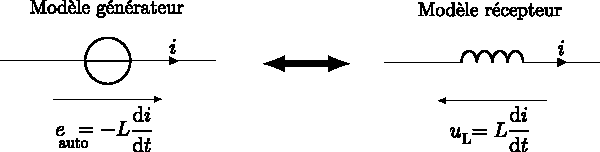
\includegraphics[scale=1]{faraequiv}
		\label{fig:faraequiv}
	\end{center}
\end{hide}
\textbf{En absence d'autres champs} que le champ propre, on peut donc remplacer
la bobine par une f.é.m.\ $e_{\rm auto}$ en convention générateur ou $u =
	-e_{\rm auto}$ en convention récepteur, c'est-à-dire
\begin{hide}
	\[
		\boxed{u = L \dv{i}{t}}
	\]
\end{hide}
qui est la caractéristique courant-tension d'une bobine vue en début d'année~!

\begin{rrema}{Remarque}
	S'il y a un champ extérieur, on applique la superposition des champs
	magnétiques~:
	\[
		\F_{\rm tot} = \F_p + \F_{\rm ext}
		\qquad
		\Ra
		\qquad
		e_{\rm tot} = -L \dv{i}{t} - \dv{\F_{\rm ext}}{t} = e_{\rm auto} + e_{\rm ext}
	\]
\end{rrema}

\section{Induction mutuelle}
\label{sec:inducmut}
\subsection{Principe de l'inductance mutuelle}
\label{ssec:prpeinducmut}
\noindent
\begin{minipage}[t]{.6\linewidth}
	Soit deux circuits fixes indépendants électriquement, sans champ magnétique
	extérieur.
	\begin{itemize}[label=$\diamond$, leftmargin=10pt]
		\item Le circuit (1) est parcouru par un courant $i_1$ qui génère un champ
		      magnétique $\vv{B_1}$~;
		\item Le circuit (2) est parcouru par un courant $i_2$ qui génère un champ
		      magnétique $\vv{B_2}$.
	\end{itemize}
	Le champ magnétique total est
	\[
		\vv{B} = \vv{B_1} + \vv{B_2} + \underbracket{\vv{B_{\rm ext}}}_{=\vv{0}}
	\]
\end{minipage}
\hfill
\begin{minipage}[t]{.4\linewidth}
	~
	\vspace*{-20pt}
	\begin{center}
		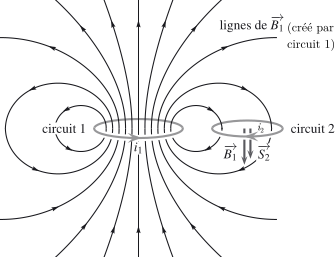
\includegraphics[width=\linewidth]{inducmut}
		\label{fig:inducmut}
	\end{center}
\end{minipage}
\textbf{En supposant les champs uniformes}, le flux magnétique total traversant
le circuit (1) est donc~:
\begin{hide}
	\begin{gather*}
		\F_1 = \vv{B}\cdot \vv{S_1} = \left(\vv{B_1}+\vv{B_2}\right)\cdot \vv{S_1}
		= \vv{B_1}\cdot \vv{S_1}+\vv{B_2}\cdot \vv{S_2}
		\\\Lra
		\F_1 = \F_{p,1} + \F_{2\ra 1}
	\end{gather*}
\end{hide}
Avec $\F_p$ le flux propre de chaque circuit, et $\F_{2\ra 1}$ le flux de
$\vv{B_2}$ à travers le circuit (1). De même, en inversant les rôles de (1) et
(2)~:
\begin{hide}
	\[
		\F_2 = \F_{p,2} + \F_{1\ra 2}
	\]
\end{hide}

\begin{tprop}{Propriété, hand}
	\cswitch{white}{
		Les flux croisés sont proportionnels au courant les générant, même dans un cas
		non-uniforme, et le coefficient de proportionnalité est \textbf{le même pour
			les deux flux}, et s'appelle \textbf{coefficient d'inductance mutuelle} $M$,
		mesuré en henry~:
		\[
			\boxed{\F_{2\ra 1} = Mi_2}
			\qqet
			\boxed{\F_{1\ra 2} = Mi_1}
		\]
		\vspace*{-10pt}
	}
\end{tprop}

\begin{rrema}{Remarque}
	Au contraire de $L$ toujours positive, $M$ peut être positif ou négatif selon
	l'orientation relative des deux circuits.
\end{rrema}

\paragraph*{Forces électromotrices}
Soit deux circuits non connectés mais en inductance mutuelle.
\begin{figure}[h]
	\centering
	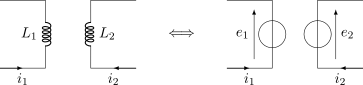
\includegraphics[scale=1]{inducmutelec}
	\label{fig:inducmutelec}
\end{figure}
\smallbreak
\noindent
Chaque circuit vérifie la loi de \textsc{Faraday}~:
\begin{hide}
	\begin{gather*}
		e_1 = - \dv{\F_1}{t} = -\dv{\F_{p,1}}{t} - \dv{\F_{2\ra 1}}{t}
		\qqet
		e_2 = - \dv{\F_2}{t} = -\dv{\F_{p,2}}{t} - \dv{\F_{1\ra 2}}{t}
	\end{gather*}
\end{hide}
\noindent
\begin{hide}
	\begin{gather*}
		\left\{
		\begin{aligned}{}
			\F_{p,1}    & = L_1i_1
			\\
			\F_{2\ra 1} & = Mi_2
		\end{aligned}
		\right.
		\qqet
		\left\{
		\begin{aligned}{}
			\F_{p,2}    & = L_2i_2
			\\
			\F_{1\ra 2} & = Mi_1
		\end{aligned}
		\right.
	\end{gather*}
\end{hide}
\noindent
Ainsi,
\begin{hide}
	\[
		\boxed{e_1 = -L_1 \dv{i_1}{t} - M \dv{i_2}{t}}
		\qqet
		\boxed{e_2 = -L_2 \dv{i_2}{t} - M \dv{i_1}{t}}
	\]
\end{hide}

\subsection{Bobines imbriquées}
\label{ssec:inducmutimbriq}
On souhaite déterminer l'inductance mutuelle de 2 bobines de même axe, de
longueurs $\ell_{i}$ et de rayons $R_{i}$, parcourues par des intensités $i_{i}$
dirigées dans le même sens. On s'intéresse d'abord à $\F_{2\ra 1}$, le flux créé
par la seconde bobine dans la première.
\begin{figure}[h]
	\centering
	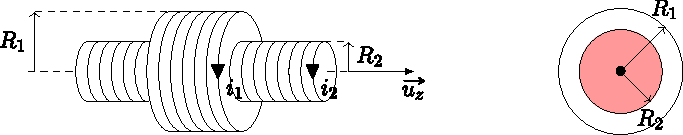
\includegraphics[scale=1]{bobimbriq}
	\label{fig:bobimbriq}
\end{figure}

\paragraph*{Expression du champ magnétique $\vv{B_2}$}~
\begin{hide}
	Le champ magnétique d'une bobine est uniforme en son sein, et négligeable en
	dehors, soit
	\[
		\vv{B_2} =
		\left\{
		\begin{array}{lr}
			\DS
			\mu_0 \frac{N_2}{\ell_2}i_2\,\uz \quad & \text{à l'intérieur}
			\\
			\vv{0} \quad                           & \text{à l'extérieur}
		\end{array}
		\right.
	\]
\end{hide}

\paragraph*{Flux de $\vv{B_2}$ à travers de $\vv{S_1}$}~
\begin{hide}
	On oriente $\vv{S_1}$ à partir de $i_1$ par la règle de la main droite~:
	\[
		\vv{S_1} = S_1\uz
	\]
	Or, le champ $\vv{B_2}$ est nul entre $S_2$ et $S_1$, d'où~:
	\begin{align*}
		\F_{2\ra 1} & = \mu_0 \frac{N_2}{\ell_2}i_2 \times S_2\times N_1
		+ 0\times (S_2-S_1) \times N_1
		\\\Lra
		\F_{2\ra 1} & = \mu_0 \frac{N_1N_2S_2}{\ell_2} i_2
		\\\Ra
		\Aboxed{M   & = \mu_9 \frac{N_1N_2S_2}{\ell _2}}
	\end{align*}
\end{hide}

\paragraph*{Calcul de $\F_{1\ra 2}$}~
\begin{hide}
	Le calcul direct et réel est plus compliqué, puisque les lignes de champs
	sortent en réalité de la première bobine et ne sont plus parallèles. On
	pourrait se contenter d'utiliser l'inductance mutuelle pour exprimer
	directement
	\[
		\F_{1\ra 2} = Mi_1
	\]
	Cependant, avec l'hypothèse de $\vv{B}$ nul en-dehors des bobines, soit
	\[
		\vv{B_1} =
		\left\{
		\begin{array}{lr}
			\DS
			\mu_0 \frac{N_1}{\ell_1}i_1\,\uz \quad & \text{à l'intérieur}
			\\
			\vv{0} \quad                           & \text{à l'extérieur}
		\end{array}
		\right.
	\]
	et toujours avec
	\[
		\vv{S_2} = S_2\uz
	\]
	on voit que la seconde bobine est traversée par $\vv{B_1}$ sur une fraction de
	sa longueur, en l'occurrence $N_2\times \frac{\ell _1}{\ell _2}$. Ainsi,
	\begin{align*}
		\F_{1\ra 2} & = \mu_0 \frac{N_1}{\cancel{\ell _1}}i_1\times
		S_2 \times N_2\frac{\cancel{\ell _1}}{\ell _2}
		\\\Lra
		\F_{1\ra 2} & = \mu_0 \frac{N_1N_2S_2}{\ell _2}i_1
	\end{align*}
	Et on retrouve bien $M$.
\end{hide}

\begin{rrema}{Remarque}
	Si les deux bobines sont de même longueur et même section, alors
	\[
		M = \mu_0 \frac{N_1N_2}{\ell }S
	\]
	avec
	\[
		L_1 = \mu_0 \frac{N_1{}^{2}}{\ell }S
		\qqet
		L_2 = \mu_0 \frac{N_2{}^{2}}{\ell }S
	\]
	Soit
	\[
		\boxed{M = \sqrt{L_1L_2}}
	\]
	On parle alors d'«~influence totale~».
\end{rrema}

\subsection{Circuits électriques couplés par inductance mutuelle}
\label{ssec:inducmutcpl}

\begin{tprop}{Méthode, heart}
	\begin{enumerate}
		\item \cswitch{white}{
			      Remplacer les inductances par leur f.é.m.\ en \textbf{convention
				      générateur}~;
		      }
		\item \cswitch{white}{
			      Appliquer la loi des mailles pour obtenir les équations électriques~;
		      }
		\item \cswitch{white}{
			      Utiliser la loi de \textsc{Faraday} et exprimer les flux magnétiques en
			      fonction des courants~;
		      }
		\item \cswitch{white}{
			      Résoudre les équations obtenues.
		      }
	\end{enumerate}
\end{tprop}

\subsubsection{Étude du circuit}
\label{ssec:mutcpletude}
\noindent
\begin{minipage}[t]{.49\linewidth}
	On étudie le circuit ci-dessous présentant un couplage par induction de deux
	circuits. Le sens de $i_1$ est imposé par le générateur, et le sens de $i_2$ est
	conventionnel (selon sa direction, $M$) sera positif ou négatif.
\end{minipage}
\hfill
\begin{minipage}[t]{.49\linewidth}
	~
	\vspace*{-40pt}
	\begin{center}
		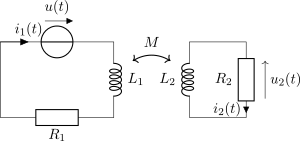
\includegraphics[scale=1]{cplmut_a}
		\label{fig:cplmut_a}
	\end{center}
\end{minipage}
\smallbreak

\paragraph*{Circuit équivalent}
\cswitch{white}{
	On remplace les bobines par des générateurs, fléchés en convention générateur
	(à partir du sens de $i_1$ et $i_2$), de forces électromotrices $e =
		-\dd{\F}/\dd{t}$~:
}
\begin{figure}[h]
	\centering
	\switch{
		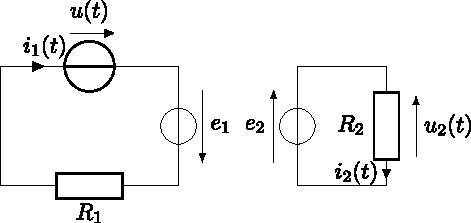
\includegraphics[scale=1]{cplmut_b}
		\label{fig:cplmut_b}
	}{
		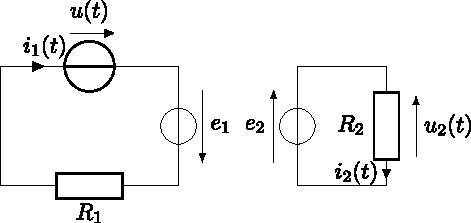
\includegraphics[scale=1, draft=true]{cplmut_b}
		\label{fig:cplmut_b}
	}
\end{figure}
\vspace*{-10pt}

\paragraph*{Équations électriques}~
\smallbreak
\noindent
\begin{minipage}[t]{.5\linewidth}
	\begin{center}
		Sur le circuit 1~:
	\end{center}
	\vspace*{-10pt}
	\cswitch{white}{
		\[
			u + e_1 = R_1i_1
		\]
	}
\end{minipage}
\hfill
\begin{minipage}[t]{.5\linewidth}
	\begin{center}
		Sur le circuit 2~:
		\vspace*{-10pt}
	\end{center}
	\cswitch{white}{
		\[
			e_2 = R_2i_2
		\]
	}
\end{minipage}

\paragraph*{Flux magnétiques et forces électromotrices}~
\smallbreak
\noindent
\begin{minipage}[t]{.5\linewidth}
	\begin{center}
		Sur le circuit 1~:
	\end{center}
	\vspace*{-20pt}
	\cswitch{white}{
		\begin{gather*}
			\F_1 = L_1i_1 + Mi_2
			\\\Ra
			e_1 = -\dv{\F_1}{t} = -L_1 \dv{i_1}{t} - M \dv{i_2}{t}
		\end{gather*}
		\vspace*{-10pt}
	}
\end{minipage}
\hfill
\begin{minipage}[t]{.5\linewidth}
	\begin{center}
		Sur le circuit 2~:
	\end{center}
	\vspace*{-20pt}
	\cswitch{white}{
		\begin{gather*}
			\F_2 = L_2i_2 + Mi_1
			\\\Ra
			e_2 = -\dv{\F_2}{t} = -L_2 \dv{i_2}{t} - M \dv{i_1}{t}
		\end{gather*}
		\vspace*{-10pt}
	}
\end{minipage}

\paragraph*{Équations couplées}~
\smallbreak
\noindent
\begin{minipage}[t]{.5\linewidth}
	\begin{center}
		Sur le circuit 1~:
	\end{center}
	\vspace*{-10pt}
	\cswitch{white}{
		\[
			R_1i_1 + L_1 \dv{i_1}{t} + M \dv{i_2}{t} = u
		\]
	}
\end{minipage}
\hfill
\begin{minipage}[t]{.5\linewidth}
	\begin{center}
		Sur le circuit 2~:
	\end{center}
	\vspace*{-10pt}
	\cswitch{white}{
		\[
			R_2i_2 + L_2 \dv{i_2}{t} + M \dv{i_1}{t} = 0
		\]
	}
\end{minipage}
Ainsi, en l'absence de couplage ($M = 0$), on retrouve les équations d'un
circuit RL classique. Avec le couplage, on peut résoudre ces équations en
passant en RSF~:
\cswitch{white}{
	\[
		(R_1 + \jj L_1 \w)\ul{I_1} + \jj M \w \ul{I_2} = \ul{U}
		\qqet
		(R_2 + \jj L_2\w)\ul{I_2} + \jj M\w \ul{I_1} = 0
	\]
}
On peut alors déterminer le comportement fréquentiel du circuit.

\subsubsection{Bilan énergétique}
\label{ssec:cplnrj}
Pour faire l'étude énergétique du circuit, on procède comme d'habitude en
faisant un bilan de puissance en \textbf{multipliant par $i$} les équations
obtenues par la loi des mailles, ici $i_1$ et $i_2$. À partir des équations
couplées,
\smallbreak
\noindent
\begin{minipage}[t]{.5\linewidth}
	\begin{center}
		Sur le circuit 1~:
	\end{center}
	\vspace*{-10pt}
	\cswitch{white}{
	\[
		R_1i_1{}^{2} + L_1i_1 \dv{i_1}{t} + Mi_1 \dv{i_2}{t} = ui_1
	\]
	\vspace*{-10pt}
	}
\end{minipage}
\hfill
\begin{minipage}[t]{.5\linewidth}
	\begin{center}
		Sur le circuit 2~:
	\end{center}
	\vspace*{-10pt}
	\cswitch{white}{
	\[
		R_2i_2{}^{2} + L_2i_2 \dv{i_2}{t} + Mi_2 \dv{i_1}{t} = 0
	\]
	\vspace*{-10pt}
	}
\end{minipage}
\bigbreak
\noindent
Ainsi, par somme on trouve
\begin{hide}
	\begin{align*}
		R_1i_1{}^{2} +R_2i_2{}^{2} +
		\dv{t}\left( \frac{1}{2} L_1i_1{}^{2} \right) +
		\dv{t}\left( \frac{1}{2}L_2i_2{}^{2} \right) +
		Mi_1 \dv{i_2}{t} + Mi_2 \dv{i_1}{t} =
		ui_1
		\\\Lra
		R_1i_1{}^{2} +R_2i_2{}^{2} +
		\dv{t}\left(
		\frac{1}{2}L_1i_1{}^{2} + \frac{1}{2}L_2i_2{}^{2} + Mi_1i_2
		\right) =
		ui_1
	\end{align*}
\end{hide}
\noindent
Ainsi, on met en évidence~:
\begin{itemize}[label=$\diamond$, leftmargin=10pt]
	\item $\mathcal{P}_{J} = R_1i_1{}^{2}(t) + R_2i_2{}^{2}(t)$
	      \cswitch{white}{
		      la puissance reçue par les résistances (dissipée par effet Joule)~;
	      }
	\item $\mathcal{P}_{\rm mag} = \dv{t}
		      \left(
		      \frac{1}{2}L_1i_1{}^{2} + \frac{1}{2}L_2i_2{}^{2} + Mi_1(t)i_2(t)
		      \right)$
	      \cswitch{white}{
		      la puissance magnétique stockée dans les deux circuits~;
	      }
	\item $\mathcal{P}_{g} = u(t)i_1(t)$
	      \cswitch{white}{
		      la puissance fournie par le générateur.
	      }
\end{itemize}
Dans le terme de puissance magnétique, on a~:
\begin{itemize}[label=$\diamond$, leftmargin=10pt]
	\item $L_1i_1{}^{2}/2$ est l'énergie magnétique emmagasinée dans le premier
	      circuit~;
	\item $L_2i_2{}^{2}/2$ est l'énergie magnétique emmagasinée dans le second
	      circuit~;
	\item $Mi_1i_2$ représente l'\textbf{énergie de couplage magnétique} entre les
	      deux circuits.
\end{itemize}
\begin{tror}{Bilan énergétique, hand}
	\vspace*{-10pt}
	\cswitch{white}{
	\begin{center}
		L'énergie du champ magnétique créé par deux circuits couplés par induction
		mutuelle est
	\end{center}
	\[
		\boxed{\mathcal{E}_{\rm mag} =
		\frac{1}{2}L_1i_1{}^{2} +
		\frac{1}{2}L_2i_2{}^{2} +
		Mi_1i_2
		}
	\]
	}
\end{tror}

\subsection{Applications}
\label{ssec:cplimpl}
\begin{itemize}[label=$\diamond$, leftmargin=10pt]
	\litem{Détecteur de métaux, boucles magnétiques (péages, parking)}. Une bobine
	créé un champ magnétique et, si un morceau de métal se trouve à proximité, il
	se créé un courant en son sein. Ce courant créé lui-même un champ magnétique
	qui perturbe le circuit primaire.
	\litem{Rechargement par induction (brosses à dent, portables)}. Le chargeur
	est muni d'une bobine qui créé un champ qui va induire un champ dans un second
	circuit.
	\litem{Chauffage par induction}. Le courant généré dans le second circuit
	chauffe par effet Joule.
	\litem{Transformateur électrique}. En enroulant deux bobines différentes
	autour d'un noyau de métal canalisant le flux, on peut diminuer ou augmenter
	la tension d'un circuit à l'autre.
\end{itemize}

% TODO: prendre Schweitzer schéma !!

\begin{figure}[h]
	\centering
	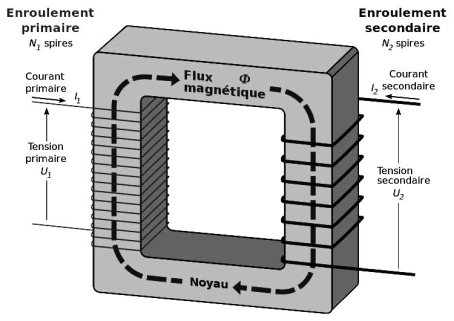
\includegraphics[scale=1]{transfo_a}
	\label{fig:transfo}
\end{figure}
Dans le modèle du transformateur parfait, on néglige toute perte par effet Joule
et le couplage est parfait~: les deux bobines sont traversées par le même flux.
Avec la loi de \textsc{Faraday} on a donc, en notant $\F(t)$ le flux du champ
dans le noyau de fer,
\[
	e_1(t) = -u_1(t) = -N_1 \dv{\F(t)}{t}
	\qqet
	e_2(t) = -u_2(t) = -N_2 \dv{\F(t)}{t}
\]
avec $N_1$ et $N_2$ le nombre de spires, et $u_1$ et $u_2$ les tensions aux
bornes du primaire et du secondaire. Ainsi,
\[
	\boxed{\frac{u_2(t)}{u_1(t)} = \frac{N_2}{N_1} = m}
\]
avec $m$ le rapport de transformation.
\begin{center}
	\danger\ Ceci n'est valable que pour un champ variable, par pour des tensions
	constantes~! \danger\
\end{center}

\end{document}

